\chapter{Control Theory II}

\newcommand{\ctii}{image/chap27_ctii}


\begin{multicols}{2}
\section{Math}
\subsection{pq-formula}
\begin{align*}
    &x^2 + px +q = 0 \\
    &x= -\frac{p}{2} \pm \sqrt{\left(\frac{p}{2}\right)^2 - q}
\end{align*}


\subsection{Exponential to trigonometric}
\begin{equation*}
   e^{i\theta} = \cos(\theta) + i\sin(\theta)
\end{equation*}


\subsection{Rank of a matrix}
The rank is the number of linear independent rows or columns.

\textbf{Method:}\newline
Step 1: Make sure that the rows or the columns are linear independent, i.e., cant multiply one row to get another row. \newline
Step 2: If there is a zero row then ignore that can not be counted. \newline
Step 3: Count the rows that are (1) linear independent and (2) non zero. \newline
\textbf{End of method}


\subsection{Transpose of matrix}
\begin{equation*}
    A^T = \left(\begin{bmatrix} a & b & c \\ d & e & f \end{bmatrix}\right)^T
    = \begin{bmatrix} a & d \\ b & e \\ c & f \end{bmatrix}
\end{equation*}


\subsection{Inverse Matrix}
\begin{align*}
    A &= \begin{bmatrix} a & b \\ c & d \end{bmatrix} \\
    A^{-1} &= \begin{bmatrix} a & b \\ c & d \end{bmatrix}^{-1} \\
    A^{-1} &= \frac{1}{ad-bc} \begin{bmatrix} d & -b \\ -c & a \end{bmatrix} \\
\end{align*}


\subsection{Determinant}
\begin{align*}
    \det{A} &= \det{\begin{bmatrix} a & b \\ c & d \end{bmatrix}} = ad-bc
\end{align*}


\subsection{Exponential and matrix exponential}
%\begin{equation*}
%    \frac{d}{dt}x e^{ax} = ae^{ax}
%\end{equation*}
%Therefore fulfills the function.
%\begin{align*}
%    \dot{f}(t) &= af(t),\; f(0) = 1\; \text{for}\; e^{ax} \\
%    \dot{F}(t) &= AF(t),\; F(0) = I\; \text{for}\; e^{Ax}
%\end{align*}
%where A is a matrix.

\begin{equation*}
    F(s)=(s I-A)^{-1} \stackrel{\mathcal{L}}{\longleftrightarrow} e^{A L}=\mathcal{L}^{-1}\left\{(s I-A)^{-1}\right\}
\end{equation*}


\textbf{Example:} Compute $e^{A_1 t}$.
\begin{equation*}
    A_1 = \begin{bmatrix} 0 & 1 \\ -1 & 0 \end{bmatrix}
\end{equation*}

\textbf{Solution}:
\begin{align*}
    sI - A_1 &= \begin{bmatrix} s & 0 \\ 0 & s \end{bmatrix} 
    - \begin{bmatrix} 0 & 1 \\ -1 & 0 \end{bmatrix} \\
    &= \begin{bmatrix} s & -1 \\ 1 & s \end{bmatrix}
\end{align*}
\begin{align*}
    (sI - A_1)^{-1} &= \left(\begin{bmatrix} s & -1 \\ 1 & s \end{bmatrix}\right)^{-1} \\
    &= \frac{1}{s^2 + 1}\begin{bmatrix} s & 1 \\ -1 & s \end{bmatrix} \\
    &= \begin{bmatrix} \frac{s}{s^2 + 1} & \frac{1}{s^2 + 1} \\ -\frac{1}{s^2 + 1} & \frac{s}{s^2 + 1} \end{bmatrix}
\end{align*}
\begin{align*}
    \mathcal{L}^{-1}((sI - A_1)^{-1}) &=  \begin{bmatrix} \cos(t) & \sin(t) \\ -\sin(t) & \cos(t) \end{bmatrix}
\end{align*}
\textbf{End of Solution}


%\textbf{WHERE SHOULD THIS BE}
%Solution to state space equation
%\begin{align*}
%    \dot{x}(t) &= ax(t) + bu(t) \\
%    X(s) &= \frac{1}{s-a}x_0 + \frac{b}{s-a}U(s) \\
%    \\
%    x(t) &= e^{at}x_0
%\end{align*}

\section{Relation between system descriptions}
\begin{figure}[H]
    \centering
    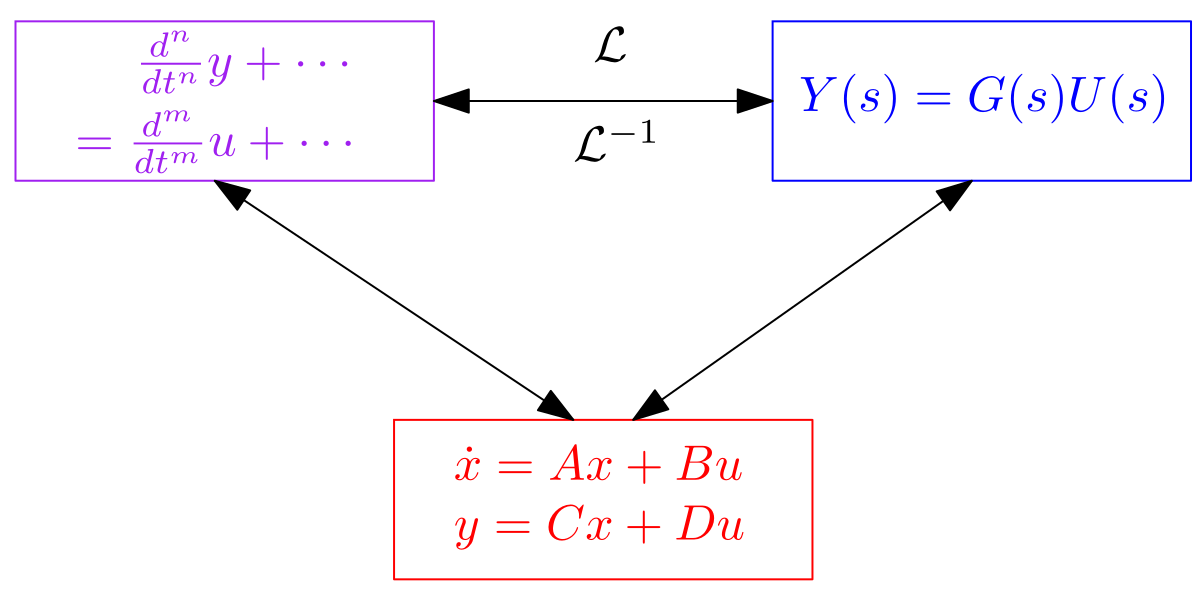
\includegraphics[width=8cm]{\ctii/relation-between-system-descriptions.png}
    \caption{Relation between system descriptions}
\end{figure}


\subsection{ODE $\rightarrow$ transfer function}
\textbf{Example:} 
Determine the transfer function of the following ODE:
\begin{equation*}
    \frac{d^2}{dt^2}{\color{blue}y} +2\frac{d}{dt}{\color{blue}y} +3{\color{blue}y} = 
    4\frac{d}{dt}{\color{red}u} +5{\color{red}u},\; {\color{red}u(t)}, y(0), \dot{y}(0) \text{ are given}
\end{equation*}

\textbf{Solution:}
\begin{align*}
    LHS = &(s^2{\color{blue}Y(s)} - sy(0) - \dot{y}(0))  \\
    &+ 2(s{\color{blue}Y(s)} - y(0)) + 3{\color{blue}Y(s)} \\
    = &(s^2 + 2s + 3){\color{blue}Y(s)} - (s+2)y(0) - \dot{y}(0)
\end{align*}
\begin{align*}
    RHS = &4(s{\color{red}U(s)} - u(0)) + 5{\color{red}U(s)} \\
    &\text{set LHS = RHS and solve } {\color{blue}Y(s)}
\end{align*}
\begin{align*}
    {\color{blue}Y(s)} = &\frac{4s+5}{s^2+2s+3}{\color{red}U(s)} \\
    &+ \frac{s+2}{s^2+2s+3}y(0) \\
    &+ \frac{1}{s^2+2s+3}(\dot{y}(0) - 4u(0))
\end{align*}
Compute ${\color{blue}y(t)} = \mathcal{L}^{-1}[Y(s)]$ using $\mathcal{L}^{-1}$ transform table 
given $\color{red}U(s) = \mathcal{L}[u(t)]$. The initial states $u(0)$, $y(0)$, and $\dot{y}(0)$
are usually set to zero unless specified otherwise.\newline
\textbf{End of Solution}


\subsection{ODE $\leftarrow$ transfer function}
Rare to go from transfer function to ODE, but it is done by 
finding the expression of $Y(s)$ and $U(s)$ and do the reverse 
of ODE to transfer function.


\subsection{ODE $\rightarrow$ State-space}
\textbf{Example:}
Determine the state-space representation of the following ODE:
\begin{equation*}
    \frac{d^2}{dt}y + 3\frac{d}{dt}y + 2y = u
\end{equation*}

\textbf{Solution:}\newline
Step 1: Express $y$ and its derivative in terms of $x_i$.
\begin{align*}
    & x_1 = y \\
    & x_2 = \frac{d}{dt}y \\
    &\Rightarrow \frac{d}{dt}x_1 = x_2
\end{align*}

Step 2: Express equation in terms of $x_i$.
\begin{align*}
    &\Rightarrow \frac{d}{dt}x_2 = -2x_1 - 3x_2 + u
\end{align*}

Step 3: Use the equation to determine the matrixes.
\begin{align*}
   &\frac{d}{dt}x = Ax + Bu  \\
   &y = Cx + Du 
\end{align*}
\begin{align*}
   &\frac{d}{dt}x = \begin{bmatrix} 0 & 1 \\ -2 & -3 \end{bmatrix}x + \begin{bmatrix} 0 \\ 1 \end{bmatrix}u  \\
   &y = \begin{bmatrix} 1 & 0 \end{bmatrix} x
\end{align*}
\textbf{End of Solution}


\subsection{ODE $\leftarrow$ State-space}
Just reverse steps of ODE to state-space.


\subsection{State-space form $\rightarrow$ transfer function}
\begin{equation*}
\left\{\begin{array} { l } 
    { {\color{burgundy}\dot{x}} = A {\color{burgundy}x} + B {\color{red}u} } \\
    { {\color{blue}y} = C {\color{burgundy}x} + D {\color{red}u} }
    \end{array} \stackrel { \mathcal { L } } { \longleftrightarrow } \left\{\begin{array}{l}
    s {\color{burgundy}X(s)} = A {\color{burgundy}X(s)} + B {\color{red}U(s)} \\
    {\color{blue}Y(s)}=C {\color{burgundy}X(s)} + D {\color{red}U(s)}
    \end{array}\right.\right.
\end{equation*}
\begin{equation*}
\left\{\begin{array}{l} % we move over  X(s) from HL
    ({\color{burgundy}s}I - A){\color{burgundy}X(s)} = B {\color{red}U(s)} \\
    {\color{blue}Y(s)}=C {\color{burgundy}X(s)} + D {\color{red}U(s)}
    \end{array}\right.
\end{equation*}
Note: we are assuming that the initial conditions are zero.

\begin{equation*}
\left\{\begin{array}{l}
    {\color{burgundy}X(s)} = ({\color{burgundy}s} I - A)^{-1} B {\color{red}U(s)} \\
    {\color{blue}Y(s)}=(C ({\color{burgundy}s}I-A)^{-1}B + D) {\color{red}U(s)}
    \end{array}\right.
\end{equation*}
Where $(C ({\color{burgundy}s}I-A)^{-1}B + D) = G(s)$ since ${\color{blue}Y(s)} = G(s){\color{red}U(s)}$.


\subsection{State-space form $\leftarrow$ transfer function}
\begin{figure}[H]
    \centering
    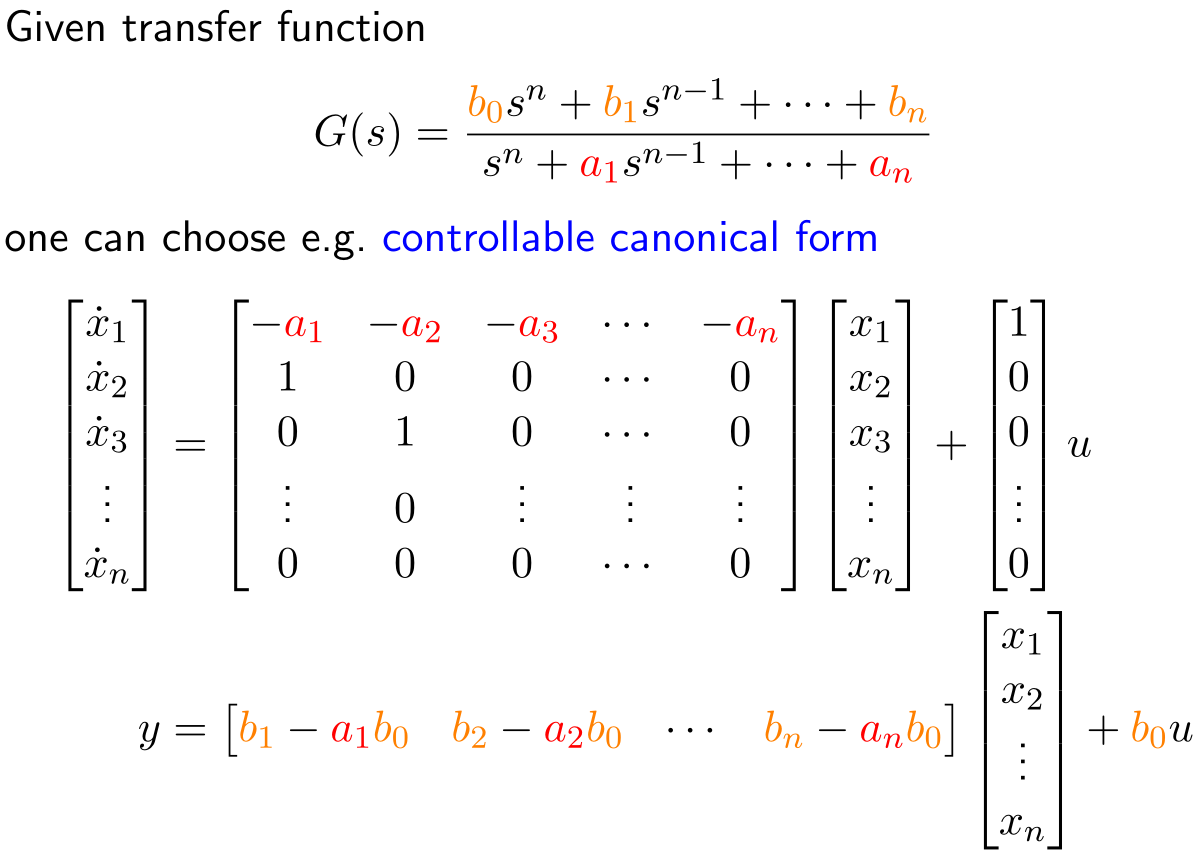
\includegraphics[width=8cm]{\ctii/controllable-canonical-form.png}
    \caption{Controllable canonical form}
\end{figure}

\begin{figure}[H]
    \centering
    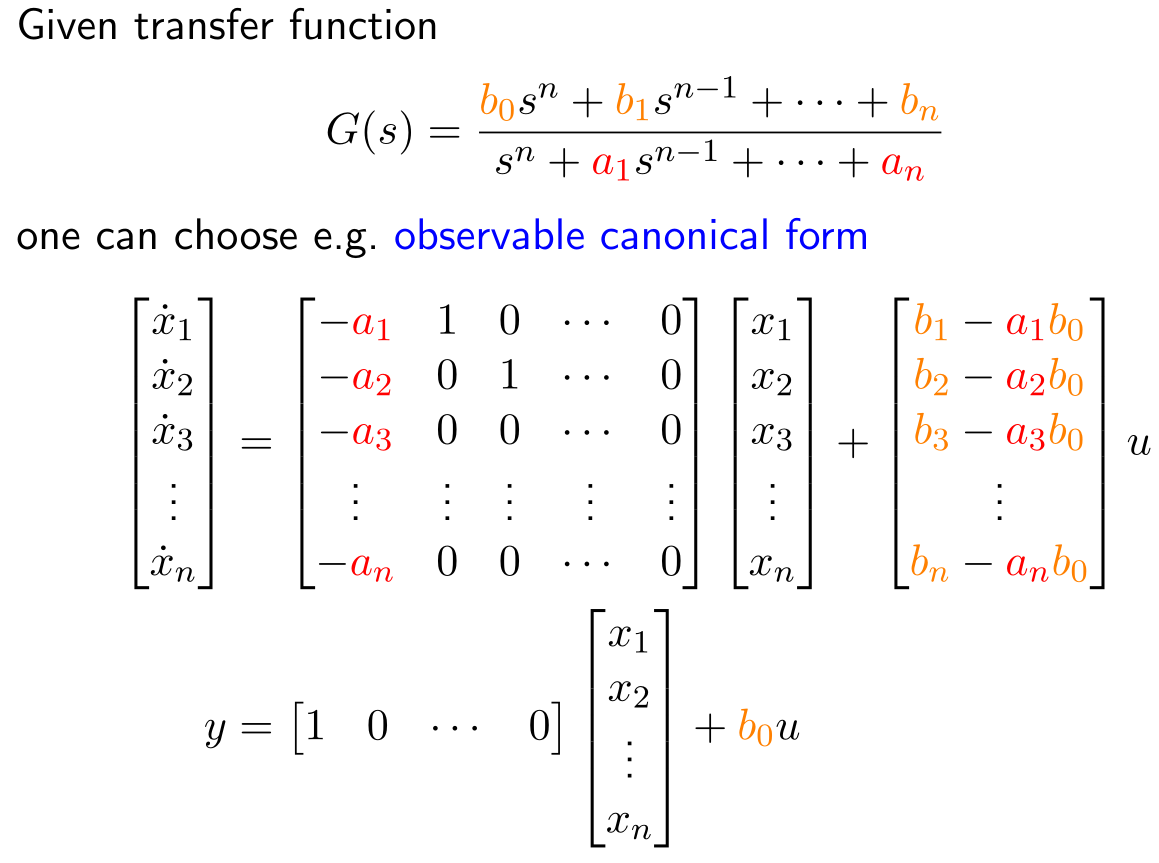
\includegraphics[width=8cm]{\ctii/observable-canonical-form.png}
    \caption{Observable canonical form}
\end{figure}


\subsection{State-space $\rightarrow$ block diagram}
\textbf{Example:}
Provide a block diagram of the following state-space representation:
\begin{align*}
    \begin{bmatrix} px_1 \\ px_2 \end{bmatrix} &= 
    \begin{bmatrix} -0.1 & 0.8 \\ 1 & 0 \end{bmatrix}
    \begin{bmatrix} x_1 \\ x_2 \end{bmatrix} 
    +\begin{bmatrix} 1 \\ 0 \end{bmatrix}u, \\
    y &= \begin{bmatrix} 1 & 0 \end{bmatrix}
    \begin{bmatrix} x_1 \\ x_2 \end{bmatrix} 
    +u.
\end{align*}

\textbf{Solution:}
\begin{align*}
    &\begin{cases}
        px_1 = -0.1x_1 + 0.8x_2 + u \\
        px_2 = x_1
    \end{cases} \\
    &\begin{cases}
        (p + 0.1)x_1 = 0.8x_2 + u \\
        x_2 = \frac{1}{p}x_1
    \end{cases} \\
    &\begin{cases}
        x_1 = \frac{0.8}{p + 0.1}x_2 + \frac{1}{p + 0.1}u \\
        x_2 = \frac{1}{p}x_1
    \end{cases}
\end{align*}

\begin{figure}[H]
    \centering
    \begin{subfigure}[b]{0.24\textwidth}
        \centering
        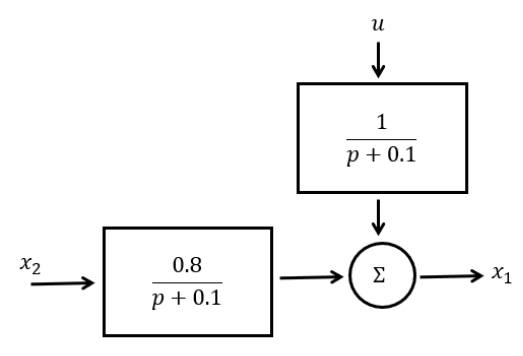
\includegraphics[width=\textwidth]{\ctii/block_diagram_example_x1.png}
        \caption{}
    \end{subfigure}
    \hfill
    \begin{subfigure}[b]{0.24\textwidth}
        \centering
        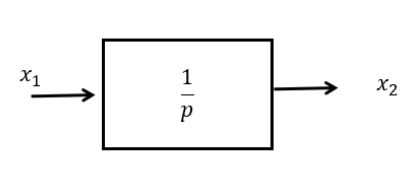
\includegraphics[width=\textwidth]{\ctii/block_diagram_example_x2.png}
        \caption{}
    \end{subfigure}
    \caption{}
\end{figure}

\begin{figure}[H]
    \centering
    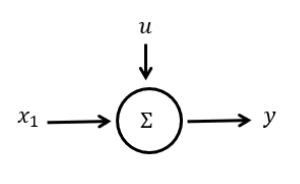
\includegraphics[width=4cm]{\ctii/block_diagram_example_y.png}
    \caption{}
\end{figure}

\begin{figure}[H]
    \centering
    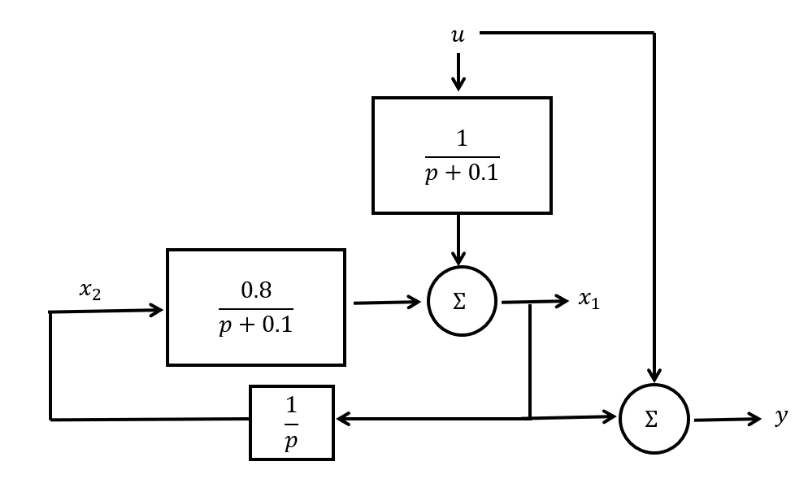
\includegraphics[width=8cm]{\ctii/block_diagram_example.png}
    \caption{Combining block diagrams}
\end{figure}
\textbf{End of solution}


\section{Controller design}
\begin{figure}[H]
    \centering
    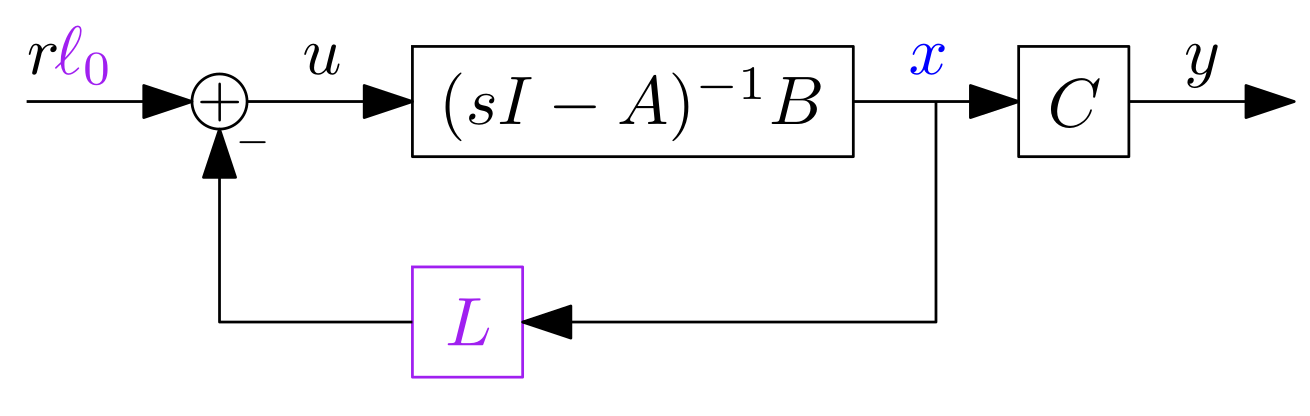
\includegraphics[width=8cm]{\ctii/state-feedback-control.png}
    \caption{State-feedback control}
\end{figure}

\begin{align*}
    \dot{x} &= (A-BL)x + Bl_0 r \\
    y &= Cx
\end{align*}


\subsection{Method: Design of state-feedback control}
\begin{equation*}
    G_c(s) = C(sI-A+BL)^{-1}Bl_0
\end{equation*}
System matrix is then:
\begin{equation*}
    (A+BL)
\end{equation*}

We can then get the eigenvalues/poles 
\begin{equation*}
    \det(sI-A+BL) = 0
\end{equation*}
Design L so that the equation holds true.

All that is left it to design $l_0$
For accuracy, it is desirable to have $G_c(0)=1$
\begin{equation*}
    l_0=\frac{1}{C(-A+BL)^{-1}B}
\end{equation*}

State-space form is controllable $\Leftrightarrow$ $L$ can be design to yield a arbitrarily placed poles (real and complex-conjugated) of the closed loop system.
$L$ solved by $\det(sI-A+BL)=0$ with designed poles.

%\textbf{Example:} TODO
%\textbf{Solution:}
%\textbf{End of solution:}


%\subsection{Closed-loop system with observer (TODO ex5)}


\subsection{Unknown states: estimate via observer}
A \textit{Observer} is an estimator with a correction term $K(y-C\hat{x})$.
\begin{equation*}
    \hat{\dot{x}} = A\hat{x} + Bu + K(y-C\hat{x}), \; \hat{x}(0) = \hat{x}_0
\end{equation*}

\begin{equation*}
    K = \begin{bmatrix} k_1 \\ k_2 \\ \vdots \\ k_n \end{bmatrix}
\end{equation*}

\begin{figure}[H]
    \centering
    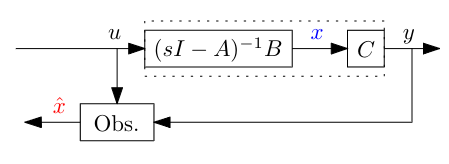
\includegraphics[width=8cm]{\ctii/observer.png}
    \caption{Observer}
\end{figure}

\begin{equation*}
    \tilde{x} \triangleq x - \hat{x}
\end{equation*}

Errors of observer described as system
\begin{equation*}
    \tilde{x}(t) = e^{(A-KC)t}\tilde{x}(0)
\end{equation*}
and therefore $||\tilde{x}(t)||$ decays at a rate given by maximum $Re\{\tilde{s}_i\}$
where $\tilde{s}_i$ are observer poles/eigenvalues of $(A-KC)$.

State-space form is observable $\Rightarrow$ matrix $K$ can be chosen such that $\tilde{x}$ vanish arbitrarily quickly.
$K$ is solved with $\det(sI - A + KC) = 0$


\subsection{Controller using estimated states}
\begin{figure}[H]
    \centering
    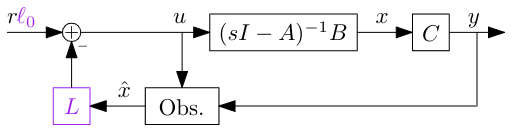
\includegraphics[width=8cm]{\ctii/feedback-with-observer.png}
    \caption{Feedback with observer}
    \label{fig:feedback-with-observer}
\end{figure}


\begin{equation*}
\left\{\begin{array} { l } 
    { \dot{x} = Ax + Bu } \\
    { y = Cx }
    \end{array} \text{and} \left\{\begin{array}{l}
    u = -L\hat{x} + l_0 r \\
    \dot{\hat{x}} = A\hat{x} + Bu + K(y-C\hat{x})
    \end{array}\right.\right.
\end{equation*}



\subsection{Closed-loop system with estimated states}
Figure~\ref{fig:feedback-with-observer} yields the closed-loop system:
\begin{align*}
    \dot{x} &= (A-BL)x + BL\tilde{x} + Cl_0r  \\
    y &= Cx
\end{align*}

with additional error states 
\begin{equation*}
    \dot{\tilde{x}} = (A-BL)\tilde{x} \to 0
\end{equation*}

\begin{equation*}
\begin{aligned}
    {\left[\begin{array}{c}
    \dot{x} \\
    \dot{x}
    \end{array}\right] } & =\underbrace{\left[\begin{array}{cc}
    A-B L & B L \\
    0 & A-K C
    \end{array}\right]}_{\tilde{A}}\left[\begin{array}{l}
    x \\
    \tilde{x}
    \end{array}\right]+\underbrace{\left[\begin{array}{c}
    B \\
    0
    \end{array}\right] \ell_0 r}_{\widetilde{B}} \\
    y & =\underbrace{\left[\begin{array}{ll}
    C & 0
    \end{array}\right]}_{\widetilde{C}}\left[\begin{array}{l}
    x \\
    \tilde{x}
    \end{array}\right]
\end{aligned}
\end{equation*}

This yields the transfer function from $r$ to $y$:
\begin{align*}
    G_c(s) &= \widetilde{C}(sI-\widetilde{A})^{-1}\widetilde{B} \\
    &= C(sI-A+BL)^{-1}Bl_0
\end{align*}


\section{CT signals and system}
\subsection{Stability for CT system}
\begin{equation*}
    x(t) = e^{At}x_0 + \int{t}_{0} e^{A\tau}Bu(t-\tau)d\tau
\end{equation*}
\textbf{Asymptotically stable} $u(t)\equiv0 \Rightarrow \lim_{t\to\infty}x(t) = 0$.
When A:s eigenvalues are strickle on the left half-plan $\Leftrightarrow$ system is asymptotically stable.
When A:s eigenvalues are strickle on the left half-plan $\Rightarrow$ system is input-output stable.

$G(s)$: poles $p_i \subseteq A$:s eigenvalues $\lambda_j$. 
And if it is minimal realization the all eigenvalues are poles.

\textbf{Example:}\newline
Is the system stable with transfer function 
\begin{equation*}
    \frac{1}{s^2-1}
\end{equation*}

\textbf{Solution:}\newline
No, since $s^2-1=(s+1)(s-1)$, meaning that one pole is $1$,
which is not allowed for stable systems.\newline
\textbf{End of solution:}

\textbf{Example 2:}\newline
Is the system stable with the following state-space representation
\begin{align*}
    \begin{bmatrix} qx_1 \\ qx_2 \end{bmatrix} &= 
    \begin{bmatrix} -0.1 & 0.8 \\ 1 & 0 \end{bmatrix}
    \begin{bmatrix} x_1 \\ x_2 \end{bmatrix}
    + \begin{bmatrix} 1 \\ 0 \end{bmatrix}u \\
    y &= \begin{bmatrix} 1 & 0 \end{bmatrix}
    \begin{bmatrix} x_1 \\ x_2 \end{bmatrix}
    +u
\end{align*}

\textbf{Solution:}
\begin{align*}
    \det{(\lambda I - A)} &= \det{\left(\begin{bmatrix} \lambda + 0.1 & -0.8 \\ -1 & \lambda \end{bmatrix}\right)} \\
    &=(\lambda + 0.1)\lambda - (-1)(-0.8) \\
    &=\lambda^2 + 0.1\lambda - 0.8 \\
    &\lambda = -\frac{0.1}{2} \pm \sqrt{\frac{0.1^2}{4} - \frac{-4\cdot0.8}{4}} \\
    &\lambda = -\frac{0.1}{2} \pm \frac{\sqrt{0.1^2 +4\cdot0.8}}{2} \\
    &\implies\lambda_+ \approx 0.8458,\;  \lambda_- \approx -0.9458
\end{align*}
\textbf{End of solution:}


\subsection{Controllable}
A state $x^*$ is \textit{controllable} when it can be expressed as a combination of $\mathcal{S}$.
\boxedeq{eq:ct-controllability-matrix}{\mathcal{S} = \begin{bmatrix} B & AB & \ldots & A^{n-1}B \end{bmatrix}}

All states $x^*$ are controllable $\Leftrightarrow$ $\mathcal{S}$:s columns are linearly independent.
$rank{(\mathcal{S})}=n$ or $\det{(\mathcal{S})} \neq 0$ if $\mathcal{S}$ is a matrix.
System is controllable $\Leftrightarrow$ It can be written on controllable canonical.

\textbf{Example:}
\begin{align*}
    \dot{x}(t) &= \begin{bmatrix} -2 & -1 \\ 1 & 0 \end{bmatrix}x(t) + \begin{bmatrix} 1 \\ 0 \end{bmatrix}u(t) \\
    y(t) &= \begin{bmatrix} 1 & 1 \end{bmatrix}x(t)
\end{align*}

\textbf{Solution}:
\begin{align*} 
    \mathcal{S} &= \begin{bmatrix} B & AB \end{bmatrix} \\
    AB &= \begin{bmatrix} -2 & -1 \\ 1 & 0 \end{bmatrix}\begin{bmatrix} 1 \\ 0 \end{bmatrix} = \begin{bmatrix} -2 \\ 1 \end{bmatrix} \\
    \mathcal{S} &= \begin{bmatrix} 1 & -2 \\ 0 & 1 \end{bmatrix} \Rightarrow \det\mathcal{S} = 1 \Leftrightarrow \text{ Controllable}
\end{align*}
\textbf{End of Solution}


\subsection{Observable}
\boxedeq{eq:ct-observable-matrix}{\mathcal{O} = \begin{bmatrix} C \\ CA \\ \vdots \\ CA^{n-1} \end{bmatrix}}

All states $x^*$ are observable $\Leftrightarrow$ $\mathcal{O}$:s columns are linear independent.
$rank{(\mathcal{O})}=n$ or $\det{(\mathcal{O})}$ if $\mathcal{O}$ is a matrix.

\textbf{Example:}
\begin{align*}
    \dot{x}(t) &= \begin{bmatrix} -2 & -1 \\ 1 & 0 \end{bmatrix}x(t) + \begin{bmatrix} 1 \\ 1 \end{bmatrix}u(t) \\
    y(t) &= \begin{bmatrix} 1 & 0 \end{bmatrix}x(t)
\end{align*}

\textbf{Solution}:
\begin{align*} 
    \mathcal{O} &= \begin{bmatrix} C \\ CA \end{bmatrix} \\
    CA &= \begin{bmatrix} 1 & 0 \end{bmatrix} \begin{bmatrix} -2 & -1 \\ 1 & 0 \end{bmatrix} = \begin{bmatrix} -2 & -1 \end{bmatrix} \\
    \mathcal{O} &= \begin{bmatrix} 1 & 0 \\ -2 & -1 \end{bmatrix} \Rightarrow \det\mathcal{S} = -1 \Leftrightarrow \text{ Observable}
\end{align*}
\textbf{End of Solution}


\subsection{Minimal realization}
State-space form of $G(s)$ is a minimal realization if vector x has the smallest possible dimension.
A state-space form is minimal realization $\Leftrightarrow$ controllable and observable $\Leftrightarrow$ A:s eigenvalues $=$ $G(s)$:s poles.



\section{DT signals and system}
Discrete-time (DT).
\begin{equation*}
\left\{\begin{array}{l}
    x(k+1) = Fx(k) + Gu(k) \\
    y(k) = Hx(k) + Ju(k)
    \end{array}\right.
\end{equation*}
where $F\in\mathbb{R}^{n\times n}$, $G\in\mathbb{R}^{n\times m}$,
$H\in\mathbb{R}^{p\times n}$, and $J\in\mathbb{R}^{p\times m}$.

The transfer function is defined as:
\boxedeq{eq:transfer-function}{G(q) = H(qI-F)^{-1}G + J}

Poles are calculated as follows:
\begin{equation*}
    0 = a(z) = \det(zI - F)
\end{equation*}

\begin{equation*}
   x(k) = F^k x_0 + \sum^{k-1}_{l=0} F^{k-1-l}Gu(l)
\end{equation*}

\textit{Causality}: For a causal system $y(k)$ depends only on $u(l)$ for $l \leq k$.


\subsection{$\mathcal{Z}$-transform}
\begin{equation*}
    Y(z) = \mathcal{Z}\lvert y(k) \rvert = \sum^{\infty}_{0} y(k)z^{-k}, \; z\in\mathcal{C}
\end{equation*}

\begin{align*}
    &\mathcal{Z}\lvert y(k+1) \rvert = zY(z) \\
    &\mathcal{Z}\lvert y(k-1) \rvert = z^{-1}Y(z)
\end{align*}
Note that $z$ works the same way as $q$.

\begin{itemize}
    \item Forward shift operator: $qy(x) = y(k+1)$
    \item Backward shift operator: $q^{-1}y(x) = y(k-1)$
\end{itemize}

\textbf{Example:}
\begin{align*}
    y(k) &= y(k-1) - v(k-1) + u(k-2) \\
    y(k+2) &= y(k+1) - v(k+1) + u(k) \\
    q^2y(k) &= qy(k) - qv(k) + u(k) \\
    q(q-1)y(k) &= u(k) - qv(k) \\
\end{align*}
\textbf{End of example}


\subsection{Stability for DT systems}
A discrete-time system is BIBO stable if the complex poles are less then $1$ away from origo in the complex plane.


\subsection{Controllability}
The Controllability matrix 
\boxedeq{eq:dt-controlable}{\mathcal{S} = \begin{bmatrix} G & FG & \ldots & F^{n-1}G \end{bmatrix}}
All controllable states $x^*$ lies in the range of $\mathcal{S} \Leftrightarrow x^* = \mathcal{S}U_n$.
The system is controllable if and only if $\mathcal{S}$ has ful rank.


\subsection{Observable}
\boxedeq{eq:dt-observable}{\mathcal{O} = \begin{bmatrix} H \\ HF \\ \vdots \\ HF^{n-1} \end{bmatrix}}

$\mathcal{O}$ is the observable matrix.
All Unobservable states $x^*_0$ lies in the null space of $\mathcal{O} = \mathcal{O}x^*_0 = 0$.
The system is observable if and only if $\mathcal{O}$ has full rank.



\subsection{State feedback with control}
Pure state feedback $u(k) = -Lx(k) + l_0r(k)$.
Observer based feedback $u(k) = -L\hat{x}(k) + l_0r(k)$.
Both give the same closed loop system:
\begin{align*}
    y(k) &= G_c(q)l_0r(k) \\
    G_c(q) &= H(qI-F+GL)^{-1}G = \frac{b(k)}{\alpha(k)} \\
    \alpha(k) &= \det(qI-F+GL)
\end{align*}
The observer poles can be obtained by solving $0=\beta(z)=\det(zI-F+KH)$.

\textbf{Example:}
\begin{equation*}
\left\{\begin{array}{l}
    x(k+1) = \begin{bmatrix} 1 & 1 \\ 0 & 0 \end{bmatrix}x(k) + \begin{bmatrix} 0 \\ 1 \end{bmatrix}u(k) + \begin{bmatrix} -1 \\ 0 \end{bmatrix}v(k) \\
    y(k) = \begin{bmatrix} 1 & 0 \end{bmatrix}x(k)
    \end{array}\right.
\end{equation*}
Find $L$ and $K$ in the control law $u(k) = -L\hat{x}(k) + l_0 r(k)$ such that $\alpha = (q - 0.6)^2$ and $\beta(q) = q^2$.

\textbf{Solution:} 
\begin{align*}
    &\det(zI-F+KH) = \\
    &= \det\left( \begin{bmatrix} z & 0 \\ 0 & z \end{bmatrix} - \begin{bmatrix} 1 & 1 \\ 0 & 0 \end{bmatrix} + \begin{bmatrix} k_0 \\ k_1 \end{bmatrix}\begin{bmatrix} 1 & 0 \end{bmatrix} \right) \\
    &= \det\left( \begin{bmatrix} z-1 & -1 \\ 0 & z \end{bmatrix} + \begin{bmatrix} k_0 & 0 \\ k_1 & 0 \end{bmatrix} \right) \\
    &= \det\left( \begin{bmatrix} z-1+k_0 & -1 \\ k_1 & z \end{bmatrix} \right) \\
    &= (z-1+k_0)(z) - (-1)(k_1)  \\
    &\Leftrightarrow k_0 = 1 \land k_1 = 0 \Rightarrow z^2
\end{align*}

\begin{align*}
    &\det((qI-F+GL)) \\
    &= \det\left( \begin{bmatrix} q & 0 \\ 0 & q \end{bmatrix} - \begin{bmatrix} 1 & 1 \\ 0 & 0 \end{bmatrix} + \begin{bmatrix} 0 \\ 1 \end{bmatrix}\begin{bmatrix} l_0 & l_1 \end{bmatrix} \right) \\
    &= \det\left( \begin{bmatrix} q-1 & -1 \\ 0 & q \end{bmatrix} + \begin{bmatrix} 0 & 0 \\ l_0 & l_1 \end{bmatrix} \right) \\
    &= \det\left( \begin{bmatrix} q-1 & -1 \\ l_0 & q+l_1 \end{bmatrix} \right) \\
    &= (q-1)(q+l_1) - (-1)(l_0) = q^2 + (l_1-1)q -(l_1 + l_0) \\
    &l_0=-0.2 \land l_1=0.16 \Rightarrow q^2 + 1.2q + 0.36 = (q+0.6)^2 
\end{align*}


\begin{equation*}
    L = \begin{bmatrix} 0.16 & -0.2 \end{bmatrix}, K = \begin{bmatrix} 1 \\ 0 \end{bmatrix}
\end{equation*}
\begin{equation*}
    y(k) = \frac{1}{(q-0.6)^2}l_0r(k) - \frac{q^2-0.2q+0.16}{q(q-0.6)^2}v(k)
\end{equation*}
Chose $l_0=0.16$ to get unit static gain ($G_c(0)=1$) from $r$ to $y$.\newline
\textbf{End solution} 

\begin{align*}
    G_c(s) = C(sI-A+BL)^{-1}Bl_0 \\
    (G_c(0)=1) \implies l_0 = \frac{1}{C(-A+BL)^{-1}B} \\
\end{align*}


\subsection{ZOH}
\textbf{Example:}
Determine the ZOH model for the following continues-time system.
\begin{align*}
    \begin{cases}
    \dot{x}(t) = \begin{bmatrix} 0 & 0 \\ 1 & 0 \end{bmatrix}x(t) + \begin{bmatrix} 1 \\ 0 \end{bmatrix}u(t) \\
    y(t) = \begin{bmatrix} 1 & 2 \end{bmatrix}x(t)
    \end{cases}
\end{align*}

\textbf{Solution:}
Step 1: Calculate $e^{At}$.
\begin{align*}
    e^{At} &= \mathcal{L}^{-1}\left\{ (sI-A)^{-1} \right\} \\
    &= \mathcal{L}^{-1}\left\{ \left(\begin{bmatrix} s & 0 \\ 0 & s \end{bmatrix}-\begin{bmatrix} 0 & 0 \\ 1 & 0 \end{bmatrix}\right)^{-1} \right\} \\
    &= \mathcal{L}^{-1}\left\{ \left(\begin{bmatrix} s & 0 \\ -1 & s \end{bmatrix}\right)^{-1} \right\} 
    = \mathcal{L}^{-1}\left\{ \frac{1}{s^2}\begin{bmatrix} s & 0 \\ 1 & s \end{bmatrix} \right\} \\
    &= \mathcal{L}^{-1}\left\{ \begin{bmatrix} \frac{1}{s} & 0 \\ \frac{1}{s^2} & \frac{1}{s} \end{bmatrix} \right\}
    = \begin{bmatrix} 1 & 0 \\ t & 1 \end{bmatrix} 
\end{align*}

Step 2: Determine $F$.
\begin{equation*}
    F = e^{At} = \begin{bmatrix} 1 & 0 \\ t & 1 \end{bmatrix}
\end{equation*}

Step 3: Determine $G$.
\begin{align*}
    G &= \int^h_0 e^{At}Bdt = \int^h_0\begin{bmatrix} 1 & 0 \\ t & 1 \end{bmatrix}\begin{bmatrix} 1 \\ 0 \end{bmatrix}dt \\
    &= \int^h_0\begin{bmatrix} 1 \\ t \end{bmatrix}dt = \left[\begin{bmatrix} t \\ \frac{1}{2}t^2 \end{bmatrix}\right]^h_0 \\
    &= \begin{bmatrix} h \\ \frac{1}{2}h^2 \end{bmatrix} \\
\end{align*}

Step 4: Determine $H$.
\begin{equation*}
    H = C = \begin{bmatrix} 1 & 2 \end{bmatrix} \\
\end{equation*}

Step 5: Use matrixes in discrete system.
\begin{align*}
    &\begin{cases}
        x(k+1) &= Fx(k) + Gu(k) \\
        y(k) &= Hx(k)
    \end{cases} \\
    &\begin{cases}
        x(k+1) &= \begin{bmatrix} 1 & 0 \\ t & 1 \end{bmatrix}x(k) + \begin{bmatrix} h \\ \frac{1}{2}h^2 \end{bmatrix}u(k) \\
        y(k) &= \begin{bmatrix} 1 & 2 \end{bmatrix}x(k)
    \end{cases}
\end{align*}
\textbf{End solution:}

\subsubsection{ZOH properties}
\begin{center}
    \begin{tabular}{ |c c c| }
        \hline
     CT system & & ZOH sampled system \\ 
        \hline
     Stable & $\Leftrightarrow$ & Stable \\ 
        \hline
     Controllable & $\Leftarrow$ & Controllable \\ 
     & $\centernot\Rightarrow$ &  \\ 
        \hline
     Observable & $\Leftarrow$ & Observable \\ 
     & $\centernot\Rightarrow$ &  \\ 
        \hline
    \end{tabular}
\end{center}

The larger the value of $a$ the faster does the system converge to a certain equilibrium
$e^{ah}$. If we want to be three times faster then $e^h$ we would get $e^{3h}$.
This works the same way with continues time if the poles are $-1$ then $-3$ is three times faster.
We can also that to convert poles from CT to DT we can simply use $e^{\text{poles in CT}h}$.
\begin{equation*}
    e^{(-2\pm i2)h} = e^{-2h} \cdot e^{\pm i2h} =  e^{-2h} (\cos{2h}\pm\sin{2h})
\end{equation*}

We need to be wary what $h$ we choice, e.g., harmonic ocillatior
$Y(s) = \frac{1}{s^2+1}U(s)$ with ZOH becomes $Y(z)=\frac{(1-\cos{h})(z+1)}{z^2-2\cos{h}z+1}U(z)$
Where choosing $h=\pi$ would give $Y(z)=0$.

Options for sampled data control.
\begin{itemize}
    \item Design $F(s)$, implement with discretized version $F_d(z)$ ("approximation").
    \item Compute $G_{ZOH}(z)$ (an exact representation of $G(s)$ for $t=kh$) and design $F(z)$.
\end{itemize}


\section{Disturbances as stochastic processes}
A \textbf{stochastic process} is sequence of random 
variables, lets call it $V$. Then the random variable 
for discrete time is $V(k)$ where $k=0,1,\ldots$
and for continues time $V(t)$ where $t\geq0$.

\textbf{Variance} refers to the spread of a data set around its mean value
and \textbf{covariance} refers to the measure of the directional relationship between two random variables.
Expectation operator
\begin{equation*}
    E[g(x)] \triangleq \int^{\infty}_{-\infty} g(x)f(x) dx
\end{equation*}
where $f(x)$ is the probability density function.
\begin{figure}[H]
    \centering
    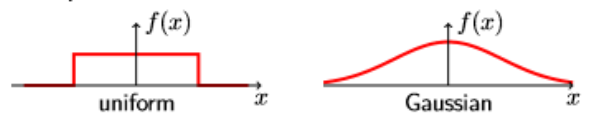
\includegraphics[width=8cm]{\ctii/probability-density-function.png}
    \caption{probability density function.}
\end{figure}

\begin{itemize}
    \item Mean: $m=E[x]$.
    \item Variance: $Var(x)=E[(x-m)^2]$.
    \item Covariance: $Cov(x,y)=E[x-m_x][y-m_y]= \int\int_{R^2}(x-m_x)(y-m_y)f(x,y)dxdy$
\end{itemize}

\textbf{Zero mean}: $E[x] = m = 0$ meaning that we standardize from the center
giving us an mean value of zero. It simplifies variance, covariance, and much more.

Covariance function of a weakly stationary stochastic process $w(t)$, with zero mean, is 
$r_w = E[w(t)w(t-\tau)^T]=E[w(t+\tau)w(t)^T]$. 
%It represents how much two variables change together.
It can be interpreted as the analogy to the the impulse response of the dynamics.
\textbf{Covariance function:}
\begin{equation*}
    r_w(\tau) \triangleq E[w(t+\tau)w(t)^T] \implies r_w(\tau) = r^T_w(-\tau)
\end{equation*} Is this true?

Properties of covariance function:
\begin{itemize}
    \item $r_w(\tau) = r_w(-\tau)^T$
    \item $r_w(0) = Var(w(t)) = E[w(t)^2]$ if scalar
    \item $r_w(0) = R_w = E[w(t)w(t)^T]$ if vector valued
    \item $|r_w(t)|\leq r_w(0)$ for all $\tau$
\end{itemize}

Covariance matrix is then $R_x = E[(x-m_x)(x-m_x)^T]\in\mathbb{R}^{n\times n}$
And for $m_x=0$, $R_x=E[xx^T]$, $R_x=R^T_x\geq0$.

White noise is a stochastic process for which $w(k)$ and $w(l)$ are independent
for every $k\neq l$. For white noise the covariance function $r_w(\tau)=0$ for all $\tau\neq0$.

\subsection{Stationary stochastic process}
A stochastic process is said to be \textbf{stationary} if its distribution is
invariant with respect to time.
This means that $w(t+\tau)$ has exactly the same probabilistic
properties for every $\tau$.

A stochastic process is said to be \textbf{weakly stationary} if its mean,
variance/covariance matrix and covariance function are invariant
with respect to time.

%A stochastic process is \textbf{stationary} if it has the same probability throughout time.
%In contrast a \textbf{weakly stationary} stochastic process has its probability space larger and larger.


\textbf{Example:}
Weakly stationary stochastic process
\begin{equation*}
    x_1(k+1) = ax_1(k) + v(k)
\end{equation*}
where $|a|<1$ and $v(k)$ is standard white Gaussian noise. 
Is it a weakly stationary stochastic process?

\textbf{Solution:}\newline
(i) zero mean:
\begin{align*}
    x(\infty) &= ax_1(\infty) + v(k) \\
    E[x(\infty)] &= aE[x_1(\infty)] + E[v(k)] \\
\end{align*}
$E[v(k)] = 0$ since it is white Gaussian noise. Therefore $E[x_1(\infty)] = 0$ 
for the equation to hold.

(ii) Variance:
State-state variance $\prod_x$ is the solution to the Lyapunov equation,
which is true if the system is asymptotically stable.
Since $|a|<1$ the system is stable.

(iii) Time-independent covariance function:
It can be solved with
\begin{equation*}
    r_x(\tau) = E[x(t+\tau)x(t)] = F^{\tau}\prod_x
\end{equation*}
Since $\prod_x$ and $F^{\tau}$ exist the covariance function is time-independent?

\textbf{End solution}

\subsection{Spectral density}
Spectral density can be interpreted as the analouge of the frequency response. \newline
\textbf{Spectral density (DT)} $-\pi\leq\omega<\pi$ % of a weakly stationary stochastic process $w(k)$ is the DFT of $r_w(\tau)$
\begin{align*}
    \Phi_w(w) &\triangleq \sum_{\tau=-\infty}^{\infty} r_{w}(\tau)e^{-i\omega\tau} \\
    &\implies  r_w(0) = \frac{1}{2\pi}\int_{-\pi}^{\pi} \Phi_w(w)dw
\end{align*}
\textbf{Spectral density (CT)} $w\in\mathbb{R}$
\begin{align*}
    \Phi_w(w) &\triangleq \int_{\tau=-\infty}^{\infty} r_{w}(\tau)e^{-i\omega\tau}d\tau \\
    &\implies r_w(0) = \frac{1}{2\pi}\int_{-\pi}^{\pi} \Phi_w(w)dw
\end{align*}

Properties of spectral density:
\begin{itemize}
%    \item $\Phi_{\omega}(\omega) = \Phi_{\omega}(-\omega)^T\geq0$
%    \item $r_{\omega}(\tau) = \frac{1}{2\pi} \int^{\pi}_{-\pi}\Phi_{\omega}(\omega)e^{i\omega\tau}d\omega$
%    \item $R_{\omega} = r_{\omega}(0) = \frac{1}{2\pi} \int^{\pi}_{-\pi}\Phi_{\omega}(\omega)d\omega$
    \item $\Phi_w(w) = \Phi^*_w(w) \geq 0$ $\forall w$
    \item ($\Phi_w(w) = \Phi_w(-w) \geq 0$ in the scalar case)
\end{itemize}
White Gaussian noise $v(k)$ has spectral density of $\Phi_v(\omega)=1$

\textbf{The spectral density for DT}
\begin{equation*}
    \Phi_z(\omega) = G(e^{i\omega})\Phi_u(\omega)G(e^{i\omega})^T
\end{equation*}

In the case of scalar:
\boxedeq{eq:spectral-density}{\Phi_z(w) = |G(e^{iw})|^2\Phi_{v_1}(w)}
where $\Phi_{v_1}(w)=1$ for white noise and $G(e^{iw})$ can be derived from $G(z) = M(zI-F)^{-1}G$ as in equation~\ref{eq:transfer-function}.
\boxedeq{eq:spectral-density-transfer-function}{|G(e^{iw})|^2 = G(e^{iw})G(e^{-iw})}

\textbf{The spectral density for CT}
\boxedeq{eq:spectral-density}{\Phi_z(w) = |G(iw)|^2\Phi_{v_1}(w)}
\boxedeq{eq:spectral-density-transfer-function}{|G(iw)|^2 = G(iw)G(-iw)}

\textbf{Example:}
\begin{equation*}
    x_1(k+1) = ax_1(k) + w(k)
\end{equation*}
where $|a|<1$ and $w(k)$ is a stochastic process that can be modeled as a 
response to standard white Gaussian noise and $v(k)$, i.e., $w(k)=G(q)v(k)$

\begin{equation*}
    \Phi(w) = \frac{0.19}{1.81-1.8\cos(w)}
\end{equation*}
Determine the transfer function $G(q)$.

\textbf{Solution:}
We know that $\Phi_z(w) = |G(e^{iw})|^2$, meaning tha the transfer function can be written as
\begin{align*}
    G(q) = \frac{a}{q+b}
\end{align*}
\begin{align*}
    |G(e^{iw})|^2 &= \frac{a}{e^{iw}+b} \frac{a}{e^{-iw}+b} \\
     &= \frac{a^2}{e^{iw-iw}+e^{iw}b+e^{-iw}b+b^2} \\
     &= \frac{a^2}{b^2 + 1 + 2b\left(\frac{e^{iw}b+e^{-iw}}{2}\right)} \\
     &= \frac{a^2}{b^2 + 1 + 2b\cos(w)} \\
\end{align*}
\begin{align*}
    \begin{cases}
        a^2 = 0.19 \implies a = \sqrt{0.19}\\
        b^2 + 1 = 1.81 \implies b = \sqrt{0.81} = \pm0.9 \\
        2b = -1.8 \implies b=\frac{-1.8}{2} = -0.9 \\
    \end{cases}
\end{align*}

Thus we have the transfer function
\begin{align*}
    G(q) =  \frac{\sqrt{0.19}}{q - 0.9}
\end{align*}

$e^{i\theta}=\cos(\theta) + i\sin(\theta)$

\textbf{End of solution}

\begin{figure}[H]
    \centering
    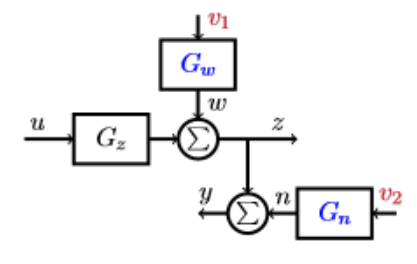
\includegraphics[width=6cm]{\ctii/disturbance-model.png}
    \caption{Disturbance model. Where $u =$ input, $z =$ controlled/performance variable, 
    $y =$ measured output, $w =$ system/process disturbance, $n =$ measurement disturbance (usually 1), 
    $v_1 =$ process noise (usually white noise), $v_2 =$ noise (usually white noise). 
    In the usually scenario $R_{12}=0$ unless specified $R_{12}=p$, and $R_{1}=R_{1}=1$.}
\end{figure}

\begin{equation*}
    \eta = \begin{bmatrix} v_1 \\ v_2 \end{bmatrix} 
    \Rightarrow \Phi_{\eta}(\omega)=R_{\eta}=
    \begin{bmatrix} R_1 & R_{12} \\ R_{12}^T & R_2 \end{bmatrix}
\end{equation*}
For scalers $R_{12} = R_{12}^T$, and for $\Phi_v(\omega)=1$ if $v$ is 
standard white noise.

\subsection{Model of stochastic processes}
Discrete:
\begin{equation*}
    \begin{cases}
        x(k+1) = Fx(k) + Gv(k) \\
        w(k) = Hx(k) + Jv(k)
    \end{cases} \end{equation*}

Continues:
\begin{equation*}
    \begin{cases}
        \dot{x}(t) = Ax(t) + Bv(t) \\
        w(t) = Cx(t) + Dv(t)
    \end{cases}
\end{equation*}

The covariance matrix $\prod_x(k) = E[x(k)x^T(k)]$ is the solution to of the\newline
Discrete-time Lyapunov equation:
\begin{equation*}
    \prod_x(k+1) = F\prod_x(k)F^T + GR_vG^T
\end{equation*}
The covariance matrix of x is
\begin{equation*}
    r_x(\tau) = E[x(k+\tau)x^{\tau}(k)] = F^{\tau}\prod_x(k), \text{ for } \tau\geq0
\end{equation*}
However, in practice we care more about the stationary condition, i.e., $k\to\infty$ which give us
the \textbf{discrete-time Laypunov equation}
\boxedeq{eq:discrete-time-lyapunov-equation}{\prod_x = F\prod_xF^T + GR_vG^T}

The \textbf{steady state variance} is denoted as $\prod_x$\newline
\textbf{Example:}
The steady state variance of 
\begin{align*}
    x(k+1) &= 
    \begin{bmatrix}
        0 & 0 \\
        0 & 0.9 \\
    \end{bmatrix}x(k) +
    \begin{bmatrix}
        1 \\
        1 \\
    \end{bmatrix} v_1(k), \\
    y(k) &= 
    \begin{bmatrix}
        1 & -1 \\
    \end{bmatrix} x(k) + v_2(k)
\end{align*}


\textbf{Solution:}
\begin{align*}
    \prod_x &= F\prod_xF^T + GR_vG^T \\
    \begin{bmatrix} 
        \pi_1 & \pi_{12} \\
        \pi_{12} & \pi_2 \\
    \end{bmatrix} &=
    \begin{bmatrix} 
        0 & 0 \\
        0 & -0.9 \\
    \end{bmatrix}
    \begin{bmatrix} 
        \pi_1 & \pi_{12} \\
        \pi_{12} & \pi_2 \\
    \end{bmatrix}
    \begin{bmatrix} 
        0 & 0 \\
        0 & -0.9 \\
    \end{bmatrix}^T \\
    &+ 
    \begin{bmatrix} 
        1 \\
        1 \\
    \end{bmatrix} 1
    \begin{bmatrix} 
        1 \\
        1 \\
    \end{bmatrix}^T \\
    \Rightarrow 
    &\begin{bmatrix} 
        \pi_1 & \pi_{12} \\
        \pi_{12} & \pi_2 \\
    \end{bmatrix} =
    \begin{bmatrix} 
        1 & 1 \\
        1 & 1+0.9^2\pi \\
    \end{bmatrix}
\end{align*}
$\Rightarrow \pi_1=\pi_{12}=1$ and $\pi_2=1+0.9^2\pi$
$\Rightarrow \pi_2=\frac{1}{1-0.9^2}\approx5.2632$

\textbf{End of solution}


The covariance matrix $\prod_x = E[x(t)x^T(t)]$ is the solution to of the\newline
Continues-time Lyapunov equation
\begin{equation*}
    \dot{\prod}_x(t) = A\prod_x(t) + \prod_x(t)A^T + BR_vB^T
\end{equation*}
And for the stationary condition the \textbf{continues-time Lyapunov equation} becomes
\boxedeq{eq:continues-time-lyapunov-equation}{0 = A\prod_x + \prod_xA^T + BR_vB^T}


The standard form 
\begin{figure}[H]
    \centering
    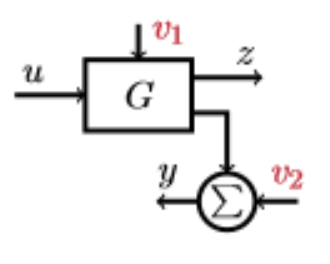
\includegraphics[width=5cm]{\ctii/disturbance-model-standard-form.png}
    \caption{Disturbance model standard form}
\end{figure}

continues time
\begin{equation*}
    \begin{cases}
        \dot{x} = Ax + Bu + Nv_1 \\
        z = Mx \\
        y = Cx + v_2
    \end{cases}
\end{equation*}

Discrete time
\begin{equation*}
    \begin{cases}
        qx = Fx + Gu + Nv_1 \\
        z = Mx \\
        y = Hx + v_2
    \end{cases}
\end{equation*}


\subsubsection{CT observer}
\boxedeq{eq:ct-observers}{\begin{split}
    \dot{\hat{x}}(t) = &A\hat{x}(t) + Bu(t) \\
    &+ K[y(t)-C\hat{x}(t)-Du(t)]
\end{split}}

If $A-KC$ is asymptotically stable then $E[\tilde{x}]=0$. And the steady state 
covariance of the estimation error is given by the continues-time lyapunov equation
\begin{equation*}
    0 = (A-KC)\prod_{\tilde{x}} + \prod_{\tilde{x}}(A-KC)^T + B_{\eta}R_{\eta}B_{\eta}^T 
\end{equation*}


\subsubsection{DT observer}
\boxedeq{eq:dt-observers}{\begin{split}
    \hat{x}(k+1) = &F\hat{x}(k) + Gu(k) \\
    &+ K[y(k)-H\hat{x}(k)-Ju(k)]
\end{split}}

If $F-KH$ is asymptotically stable then $E[\tilde{x}]=0$. And the steady state 
covariance of the estimation error is given by the continues-time lyapunov equation
\begin{equation*}
    \prod_{\tilde{x}} = (F-KH)\prod_{\tilde{x}}(F-KH)^T + G_{\eta}R_{\eta}G_{\eta}^T 
\end{equation*}


\subsection{Kalman filter}
Kalman filter is an estimator that is always stable.

\subsubsection{CT Kalman filter}
Kalman filter in CT is defined as
\boxedeq{eq:ct-estimator}{
\begin{split}
    \dot{\hat{x}}(k+1|k) = &A\hat{x}(t) + Bu(t) \\
    &+ K[y(t) -C\hat{x}(t)-Du(t)]
\end{split}
}

The optimal Observer is called the Kalman filter.
Let $P = \min\limits_{K}\prod_{\tilde{x}}$, $P=P^T\geq0$. The optimal observable gain is 
\boxedeq{eq:discrete-time-lyapunov-equation}{K = (PC^T + NR_{12})R^{-1}_{2}}

The steady state observer continues-time algebraic Riccati equation (\textbf{OCARE})
\boxedeq{eq:care}{\begin{split}
    0 = &AP + PA^T + NR_1N^T  \\
    &- (PC^T + NR_{12})R^{-1}_{2}(PC^T + NR_{12})^T
\end{split}}

where $R_2=R_2^T > 0$ and $R_{\eta} = R_{\eta}^T \geq0$, and $(A, C)$
always gives $A-KC$ is asymmetrically stable.


\subsubsection{DT Kalman filter}
Let $\hat{x}(k|l)$ be the estimate of $x(k)$ based on the measurements 
up to time $l$, i.e., $\ldots, y(l-2), y(l-1), y(l)$.
\boxedeq{eq:ct-estimator}{
\begin{split}
    \hat{x}(k+1|k) = &F\hat{x}(k|k-1) + Gu(k) \\
    &+ K[y(k) -H\hat{x}(k|k-1)-Ju(k)]
\end{split}
}

where $P=\min\limits_{K}\prod_{\tilde{x}(k|k-1)}$.
The optimal observer gain is
\boxedeq{eq:discrete-time-lyapunov-equation}{K = (FPH^T + NR_{12})(HPH^T + R_2)^{-1}}

$P = P^T \geq 0$ is the solution to the (state space) 
observer discrete-time algebraic Riccati equation (\textbf{ODARE}).
\boxedeq{eq:dare}{\begin{split}
    P = &FPF^T + NR_1N^T \\
    &-(FPH^T + NR_{12})(HPH^T+R_2)^{-1} \\
    &(FPH^T+NR_{12})^T
\end{split}}


If we wan the optimal estimator for the next step we solve
\begin{align*}
    \hat{x}(k|k) = &\hat{x}(k|k-1) \\
    &+ \tilde{K}[y(k)-H\hat{x}(k|k-1)-Ju(k)] \\
\end{align*}

If we want to predict $m$-steps predictor
\begin{align*}
    \hat{x}(k+m|k) = &F^m \hat{x}(k|k) + \sum^{m-1}_{l=0} F^{m-1-l} Gu(k+l) \\
    &F^{m-1} N\hat{v}_1(k|k) \\
    \hat{v}_1(k|k) = &R_{12}(HPH^T + R_2)^{-1}v(k), \\
    & (=0 \text{ if } R_{12}=0)
\end{align*}

The observer gain $K$ is a matrix used to minimize 
the difference between the actual output $y$ and 
the estimated output $\hat{y}$.

\textbf{Example}\newline
\begin{align*}
    x(k+1) = &\begin{bmatrix} 0 & 0 \\ 0 & 0.9 \end{bmatrix}x(k)
    +\begin{bmatrix} 1 \\ 1 \end{bmatrix}v_1(k) \\
    y(k) = &\begin{bmatrix} 1 & -1 \end{bmatrix}x(k) + v_2(k)
\end{align*}

\textbf{Solution:}\newline
Step 1: define the observer gain
\begin{equation*}
    K = (FPH^T + NR_{12})(HPH^T + R_2)^{-1}
\end{equation*}

Step 2: calculate the $P$ 
\begin{align*}
    P = &FPF^T + NR_1N^T \\
    &-(FPH^T + NR_{12})(HPH^T+R_2)^{-1} \\
    &(FPH^T+NR_{12})^T \\
    \begin{bmatrix} p_{1} & p_{12} \\ p_{12} & p_{2} \end{bmatrix}
    = 
    &\begin{bmatrix} 0 & 0 \\ 0 & -0.9 \end{bmatrix}
    \begin{bmatrix} p_{1} & p_{12} \\ p_{12} & p_{2} \end{bmatrix}
    \begin{bmatrix} 0 & 0 \\ 0 & -0.9 \end{bmatrix}\\
    &+\begin{bmatrix} 1 \\ 1 \end{bmatrix}1
    \begin{bmatrix} 1 & 1 \end{bmatrix}\\
    &-\left(
    \begin{bmatrix} 0 & 0 \\ 0 & -0.9 \end{bmatrix}
    \begin{bmatrix} p_{1} & p_{12} \\ p_{12} & p_{2} \end{bmatrix}
    \begin{bmatrix} 1 \\ -1 \end{bmatrix}
    \right)\\
    &\left(
    \begin{bmatrix} 1 & -1 \end{bmatrix}
    \begin{bmatrix} p_{1} & p_{12} \\ p_{12} & p_{2} \end{bmatrix}
    \begin{bmatrix} 1 \\ -1 \end{bmatrix} +1
    \right)^{-1}\\
    &\left(
    \begin{bmatrix} 0 & 0 \\ 0 & -0.9 \end{bmatrix}
    \begin{bmatrix} p_{1} & p_{12} \\ p_{12} & p_{2} \end{bmatrix}
    \begin{bmatrix} 1 \\ -1 \end{bmatrix}
    \right)^T
\end{align*}

This is derived to 
\begin{align*}
    \begin{bmatrix} p_{1} & p_{12} \\ p_{12} & p_{2} \end{bmatrix}
    =
    &\begin{bmatrix} 0 & 0 \\ 0 & (-0.9)^2p_2 \end{bmatrix}
    \begin{bmatrix} 1 & 1 \\ 1 & 1 \end{bmatrix}\\
    &-\frac{1}{p_1 -2p_{12} -p_2 +1} \\
    &\begin{bmatrix} 0 & 0 \\ 0 & (-0.9)^2(p_{12}-p_{2})^2 \end{bmatrix}
\end{align*}

This gives us $p_1=P_{12}=1$ and then $p_2$:
\begin{equation*}
    p_2 = (-0.9)^2p_2 + 1 - \frac{(-0.9)^2(p_{12}-p_{2})^2}{p_1 - 2p_{12} -p_2 +1}
\end{equation*}
Which is derived to $p_2^{(1)} = 0.36$, $p_2^{(2)} = 2.2619$.
Both are positive, however $p_2^{(1)}<1$, i.e., the variance is lower then the 
standard distribution noise affection the system and sensors.


Step 3: calculate the observer gain
\begin{align*}
    K &= 
    \begin{bmatrix} 
        0 & 0 \\
        0 & -9 \\
    \end{bmatrix} 
    \begin{bmatrix} 
        1 & 1 \\
        1 & 2.2619 \\
    \end{bmatrix} 
    \begin{bmatrix} 
        1  \\
        -1  \\
    \end{bmatrix} 
    \frac{1}{2.2619} \\
    &= 
    \begin{bmatrix} 
        0 \\
        0.5021 \\
    \end{bmatrix} 
\end{align*}
\textbf{End of example}

\subsubsection{Properties of Kalman filter}
\begin{itemize}
    \item Is linear 
    \item Is always stable
    \item Is the optimal linear filter 
    \item Is the optimal state estimator if $v_1$ and $v_2$ are Gaussian.
\end{itemize}


\section{LQG}
Linear Quadratic Gaussian LQG is comprised of a Kalman filter that provides 
the estimator for the LQR controller.
The Notation change between kalman filter and LQ is shown below.

$Q_1$ is for (performance).., $Q_2$ is for (energy, smaller $Q_2$ makes for faster response)..
\textbf{TODO}

%Optimal control law $u(t)=-L\hat{x}(t)$ for CT and $u(k) = -L\hat{x}(k) + \tilde{r}(k)$
%for DT, where $\hat{x}$ is obtained from corresponding Kalman filter.
%The optimal state feedback gain is 
%\boxedeq{eq:lqg-optimal-state-feedback-gain}{L = Q^{-1}_2B^TS}
%the matrix $S=S^T\geq0$ is the solution to the steady state
%control continuous-time algebraic Riccati equation (cCare).
%\boxedeq{eq:lqg-optimal-state-feedback-gain}{0 = A^TS + SA + M^TQ_1M - SBQ^{-1}_2B^TS}

\begin{table}[H]
    \centering
    \begin{tabular}{c c c c c c c c} 
    KF: & $A$            & $N$            & $C$            & $R_1$          & $R_2$          & $P$            & $K$ \\ 
        & $\updownarrow$ & $\updownarrow$ & $\updownarrow$ & $\updownarrow$ & $\updownarrow$ & $\updownarrow$ & $\updownarrow$ \\
    LQ: & $A^T$          & $M^T$          & $B^T$          & $Q_1$          & $Q_2$          & $S$            & $L^T$ \\
    \end{tabular}
\end{table}

% TODO: examples

\subsection{LQG for CT systems}
\begin{align*}
    &\begin{cases}
        \dot{x} = Ax + Bu + Nv_1 \\
        z = Mx \\
        y = Cx + v_2
    \end{cases} \\
    &\eta = \begin{bmatrix} v_1 \\ v_2 \end{bmatrix},
    \Phi_{\eta}(\omega) = \begin{bmatrix} R_1 & R_{12} \\ R^T_{12} & R_2 \end{bmatrix}
\end{align*}

Minimize the criterion
\begin{equation*}
    V = ||z||^2_{Q_1} + ||u||^2_{Q_2}
\end{equation*}

The weighting matrix that are used as design parameters.
\begin{equation*}
    Q_1 = Q_1^T \geq 0,\; Q_2 = Q_2^T \geq 0
\end{equation*}


\textbf{Optimal control law}
\boxedeq{eq:lqg-ct-optimal-control-law}{u(t) = -L\hat{x}(t)}

\textbf{Estimator} is obtained from the Kalman filter 
by equation~\ref{eq:ct-observers}.

\textbf{Optimal state feedback gain}
\boxedeq{eq:lqg-ct-optimal-state-feedback-gain}{L=Q^{-1}_2 B^T S}
where $S=S^T\geq0$ solves the control continues-time algebraic Riccati equation cCARE:
\boxedeq{eq:lqg-ct-care}{0 = A^TS + SA + M^TQ_1M - SBQ^{-1}_2B^TS}


\subsection{LQG for DT systems}
\begin{align*}
    &\begin{cases}
        qx = Fx + Gu + Nv_1 \\
        z = Mx \\
        y = Hx + v_2
    \end{cases} \\
    &\eta = \begin{bmatrix} v_1 \\ v_2 \end{bmatrix},
    \Phi_{\eta}(\omega) = \begin{bmatrix} R_1 & R_{12} \\ R^T_{12} & R_2 \end{bmatrix}
\end{align*}


\begin{itemize}
\item Minimize $V = ||z||^2_{Q_1} + ||u||^2_{Q_2}$
    \begin{itemize}
    \item $= E[z^TQ_1z + u^TQ_2u]$ (stochastic),
    \item $= \lim_{N\to\infty} \frac{1}{N}\sum^N[z^TQ_1z + u^TQ_2u]$ (empirical stoch),
    \item $= \sum^{\infty}[z^TQ_1z + u^TQ_2u]$ (deterministic).
    \end{itemize}
\item $Q_1 = Q^T_1 \geq 0$ and $Q_2 = Q^T_2 > 0$ are design parameters.
\item Control strategy $=$ observer based state feedback control:
    \begin{itemize}
    \item $q\hat{x} = F\hat{x} + Gu + K(y-H\hat{x})$
    \end{itemize}
\end{itemize}
\textbf{Optimal control law}
\boxedeq{eq:lqg-dt-optimal-control-law}{u(k) = -L\hat{x}(k|k-1)}

\textbf{Estimator} is obtained from the Kalman filter 
by equation~\ref{eq:dt-observers}.

\textbf{Optimal state feedback gain}
\boxedeq{eq:lqg-dt-optimal-state-feedback-gain}{L=(G^{T}SG + Q_2)^{-1}G^{T}SF}
where $S=S^T\geq0$ solves the DARE in equation~\ref{eq:dare}.



% TODO Theorem 9.4
\subsection{LQ/LQG: Properties}
\begin{itemize}
    \item $F-GL$ is always stable
    \item The control law $u(k) = -Lx(k)$ (pure state feedback) is optimal, also for the deterministic case ($v_1 = 0$ and $v_2 = 0$)
    $\Leftrightarrow LQ =$ linear quadratic (regulated) control.
    \item If $v_1$ and $v_2$ have Gaussian disturbance the controller is the optimal controller 
    $\Leftrightarrow LQG =$ linear quadratic gaussian control.
    \item Theorem 9.4 = the seperation theorem. The optimal observer $=$ Kalman filter, 
    combined with the optimal state feedback (LQ) give the optimal controller!
    \item The LQ/LQG controller looks exactly the same for SISO and MIMO system.
    \item The servo problem: Use $u = -L$
\end{itemize}
% TODO: servo motor problem?


\section{MPC}
The objective of Model Predictive Control (MPC) is to 
find the input which minimize the cost function through 
optimization.

System to be controlled:
\begin{align*}
    &\begin{cases}
    y(k) = G(q)u(k) + v(k), \\
    y_m(k) = y(k) + e(k)
    \end{cases}  \\
    &\begin{cases}
    |u(k)| \leq C_u, \\
    |y(k)| \leq C_y
    \end{cases}
\end{align*}

Minimizing
\begin{equation*}
    V = \sum^M_{k=1}y^T(k)Q_1y(k) + \sum^N_{k=0}u^T(k)Q_2u(k), N<M
\end{equation*}

\begin{itemize}
    \item $M$: prediction horizon
    \item $N$: control horizon
\end{itemize}

The steps that are taken model predictive control at time k.
\begin{enumerate}
    \item Measure $y_m(k)$, use a Kalman filter to get $\hat{x}(k|k)$
    \item Minimize the cost function 
    \begin{equation*}
    V_k = \sum^{k+M}_{l=k+1}\hat{y}^T(l|k)Q_1(l)y(l|k) + \sum^{k+N}_{l=k}u^T(l)Q_2(l)u(l)
    \end{equation*}
    \item Apply $u(k)$ on the system
    \item Wait for the next sample instant, $k+1$, and go to step $1$
\end{enumerate}


\subsection{MPC design parameters}
In MPC we have $Q_1$, $Q_2$, $N$, $M$, and $h$.
\begin{itemize}
    \item $Q_1$ and $Q_2$ have the same role as in LQG.
    \item $N<<M$
    \item Typically $Mh \approx T_s$
    \item The bigger $N$, the smoother control but more computation
    \item The sampling period $h$. The control horizion is $Nh$ so shorter $h$ we ger short control horizion.
\end{itemize}

\end{multicols}
